\documentclass{beamer}
\usetheme{metropolis}           % Use metropolis theme
%\usepackage{appendixnumberbeamer}

%%% Bibliography
\usepackage[backend=bibtex, style=authoryear]{biblatex}
\bibliography{bibliography.bib}

\setbeamercolor{title}{fg=white}
\setbeamercolor{author}{fg=black}
\setbeamercolor{institute}{fg=white}

\newcommand{\todo}{\alert{TODO}}

\title{Mastering the game of Go \\ with deep neural networks and tree search}
\date{}                         % no dates
\author{Karel Ha \\ article by Google DeepMind}
%\author{Google DeepMind \\ presented by Karel Ha}
\institute{Spring School of Combinatorics 2016}

\begin{document}
  {
    \usebackgroundtemplate{
      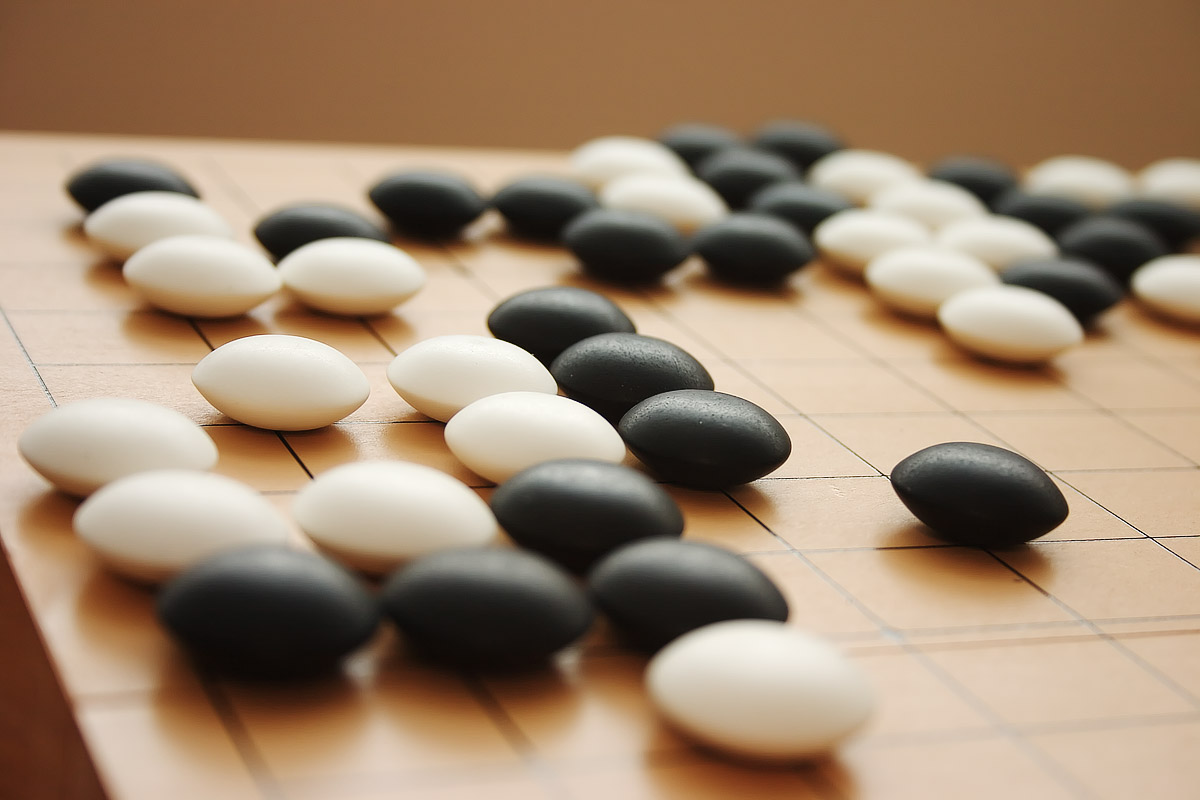
\includegraphics[height=\paperheight]{../img/Go_background.jpg}
    }
    \maketitle
  }

%%%%%%%%%%%%%%%%%%%%%%%%%%%%%%%%%%%%%%%%%%%%%%%%%%%%%%%%%%%%%%%%%%%%%%%%%%%%%%%%

  \section{Why AI?}

  \begin{frame}{Applications of AI}
    \begin{itemize}[<+- | alert@+>]
      \item spam filters
      \item predictive text (Swiftkey)
      \item self-driving cars
    \end{itemize}
    \pause

    and...
  \end{frame}

  {
    \setbeamertemplate{frame footer}{\cite{Corrado15}}
    \begin{frame}{Auto reply feature of~Google Inbox}
      \begin{center}
        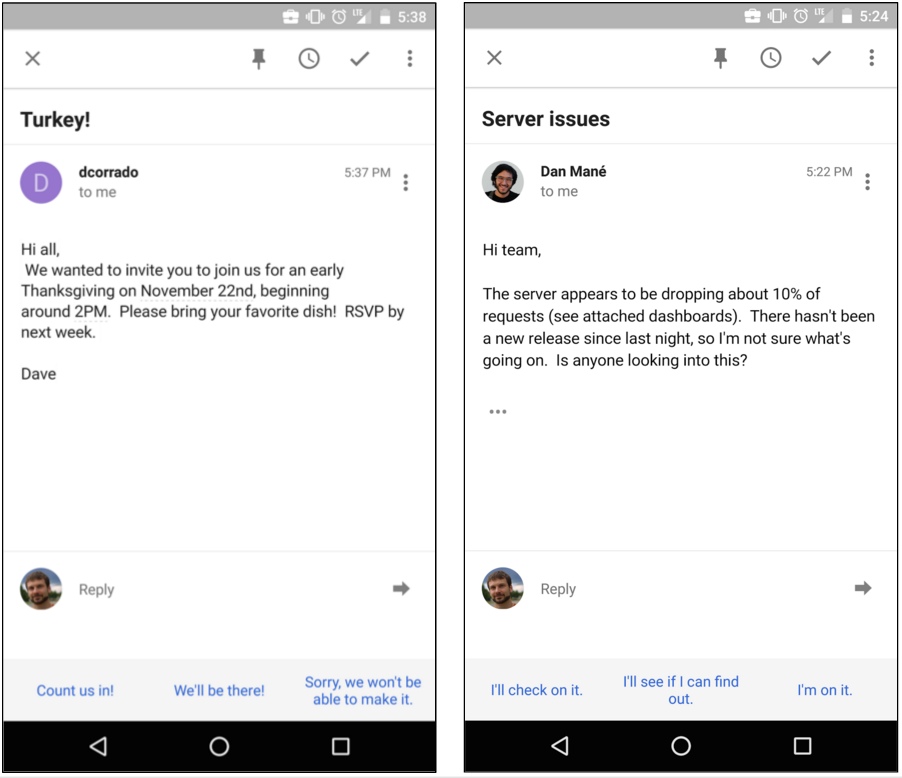
\includegraphics[height=.85\textheight]{../img/Inbox_auto_reply.png}
      \end{center}
    \end{frame}
  }

  {
    \setbeamertemplate{frame footer}{[1] \cite{GatysEB15a} [2] \cite{LiW16}}
    \begin{frame}{Artistic-style painting}
      \begin{center}
        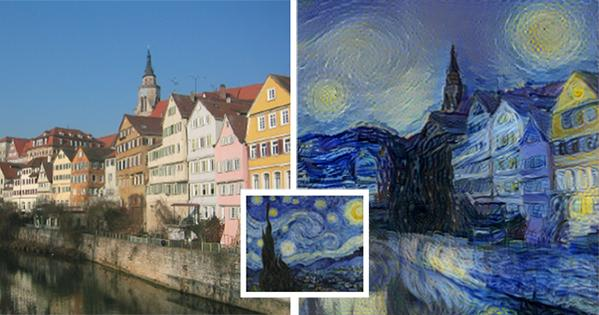
\includegraphics[height=.4\textheight]{../img/art_Van_Gogh.jpg}
        \pause

        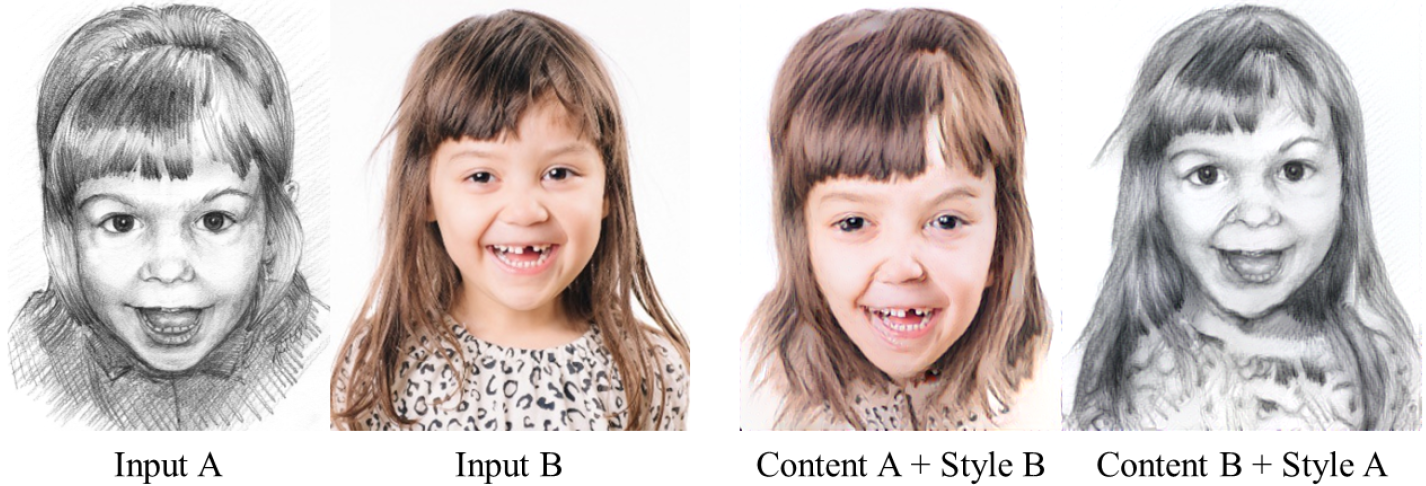
\includegraphics[height=.44\textheight]{../img/art_girl.png}
      \end{center}
    \end{frame}
  }

  {
    \setbeamertemplate{frame footer}{\cite{DeepDrumpf}}
    \begin{frame}{DeepDrumpf}
      \url{https://twitter.com/deepdrumpf}
      \pause
      - a~Twitter bot that has learned the~language of~Donald Trump from his speeches 
      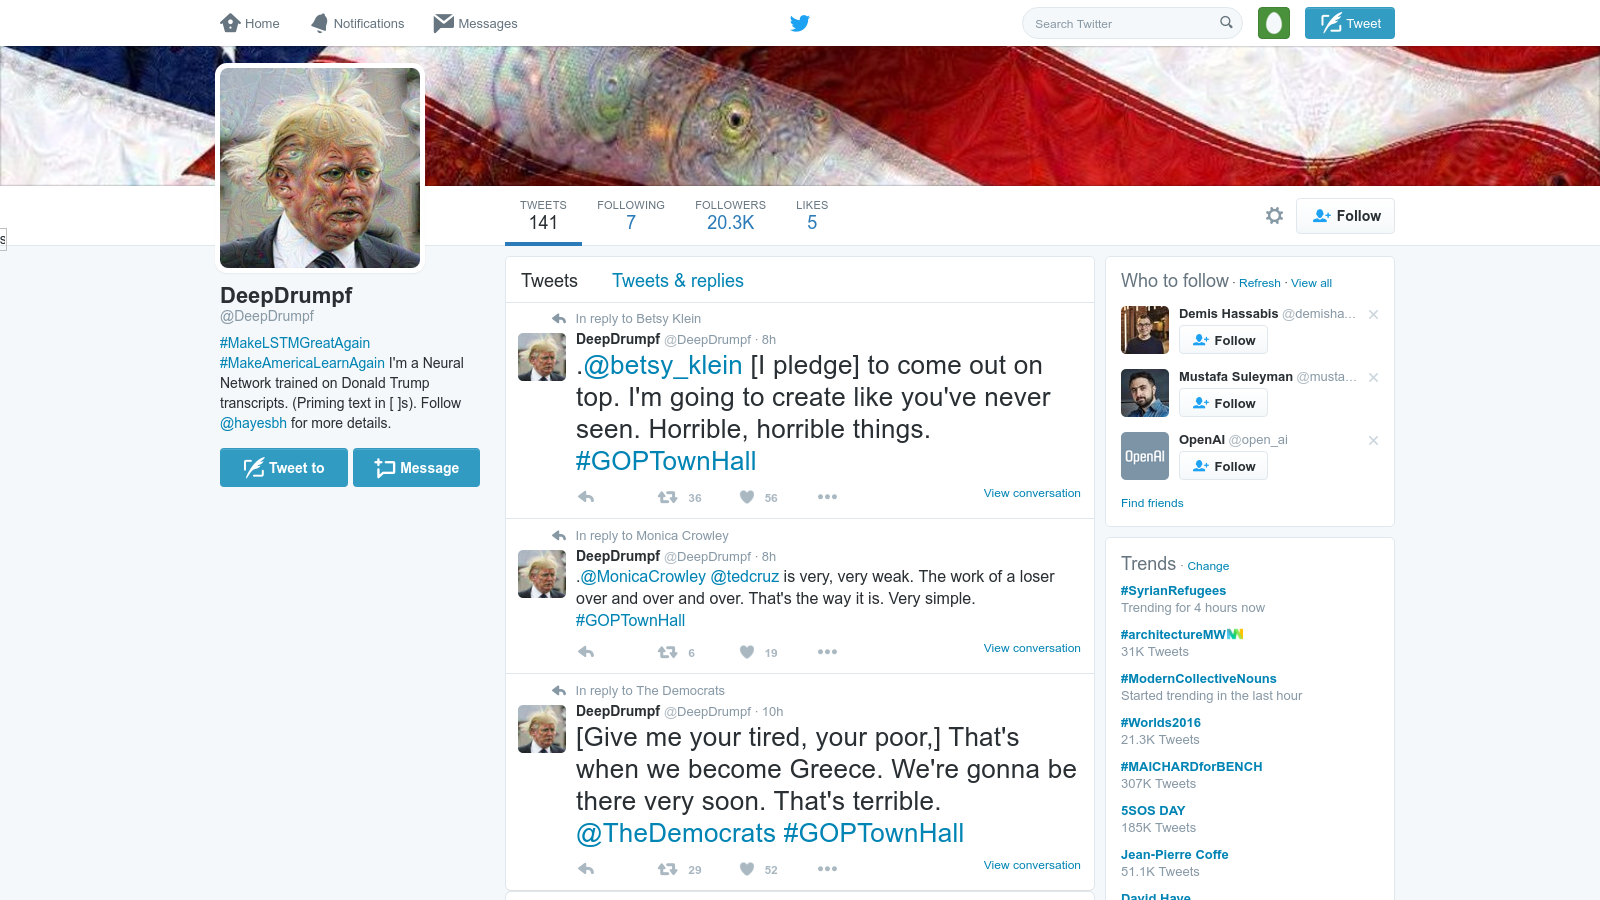
\includegraphics[width=\textwidth]{../img/DeepDrumpf.png}
    \end{frame}
  }

%%%%%%%%%%%%%%%%%%%%%%%%%%%%%%%%%%%%%%%%%%%%%%%%%%%%%%%%%%%%%%%%%%%%%%%%%%%%%%%%

  \section{Basics of Machine learning}

  \begin{frame}{Supervised versus unsupervised learning}
    Supervised learning
    \begin{itemize}[<+- | alert@+>]
      \item \todo
      \item \todo
    \end{itemize}
    \pause

    Unsupervised learning:
    \begin{itemize}[<+- | alert@+>]
      \item \todo
      \item \todo
    \end{itemize}
  \end{frame}

  \begin{frame}{Supervised learning}
    Phases:
    \pause
    \begin{enumerate}[<+- | alert@+>]
      \item data collection: Google Search, Facebook ``Likes'', Siri, Netflix, YouTube views, LHC collisions...
      \item training on~\textbf{training set}
      \item testing on~\textbf{testing set}
      \item final deployment
    \end{enumerate}
    \pause
  \end{frame}

  \begin{frame}{Regression}
    \todo
  \end{frame}

  \begin{frame}{Classification}
    \todo
  \end{frame}

  {
    \setbeamertemplate{frame footer}{\url{https://www.researchgate.net/post/How_to_Avoid_Overfitting}}
    \begin{frame}{Underfitting and overfitting}
      \begin{center}
        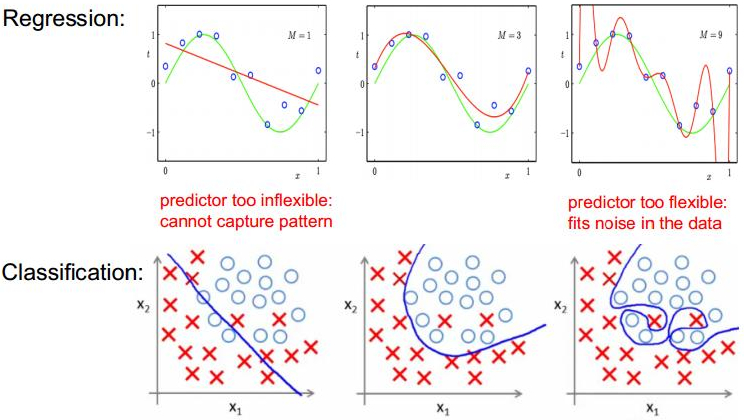
\includegraphics[width=.75\textwidth]{../img/underfitting_and_overfitting.jpg}
        \pause

        Beware of~overfitting!
      \end{center}
    \end{frame}
  }

  \begin{frame}{Reinforcement learning}
    \alert{Self-play}
    \todo
  \end{frame}

%%%%%%%%%%%%%%%%%%%%%%%%%%%%%%%%%%%%%%%%%%%%%%%%%%%%%%%%%%%%%%%%%%%%%%%%%%%%%%%%

  \section{Monte Carlo Tree Search}
  \begin{frame}{Game-tree of Go}
    \todo
  \end{frame}

%%%%%%%%%%%%%%%%%%%%%%%%%%%%%%%%%%%%%%%%%%%%%%%%%%%%%%%%%%%%%%%%%%%%%%%%%%%%%%%%

  \section{Neural networks}
  \begin{frame}{Neural network}
    \todo
  \end{frame}

  \begin{frame}{Deep neural network}
    \todo
  \end{frame}

  \begin{frame}{Convolutional neural network}
    \todo
  \end{frame}

%%%%%%%%%%%%%%%%%%%%%%%%%%%%%%%%%%%%%%%%%%%%%%%%%%%%%%%%%%%%%%%%%%%%%%%%%%%%%%%%

  \section{Rules of Go}
  \begin{frame}{Rules of Go}
    \emph{Black} versus \emph{White}.
    Black starts the game.

    \pause
    Two rules:
    \begin{description}
      \item [the rule of liberty] \todo
      \item [the ``ko'' rule] \todo
    \end{description}

    \pause
    \emph{Handicap} for difference in rank:
    Black can place 2 or more stones in advance (compensation for White's greater strength).
  \end{frame}

  \begin{frame}{Ranks}
    \todo
  \end{frame}

%%%%%%%%%%%%%%%%%%%%%%%%%%%%%%%%%%%%%%%%%%%%%%%%%%%%%%%%%%%%%%%%%%%%%%%%%%%%%%%%

  \section{AlphaGo: Inside Out}
  {
    \setbeamertemplate{frame footer}{\cite{Silver2016mastering}}
    \begin{frame}{Training the (deep convolutional) neural networks}
      \begin{center}
        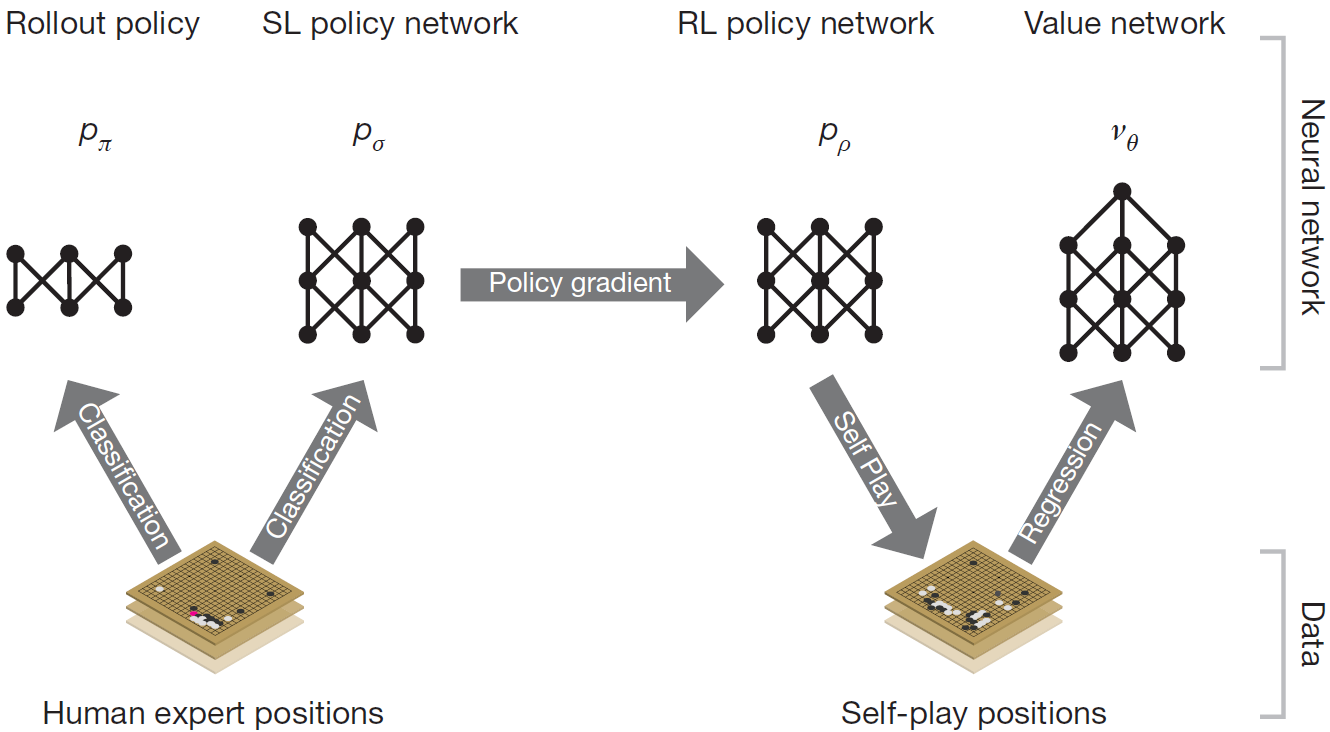
\includegraphics[width=\textwidth]{../img/neural_nets_pipeline.png}
      \end{center}
    \end{frame}

    \begin{frame}{Policy and value networks}
      \begin{center}
        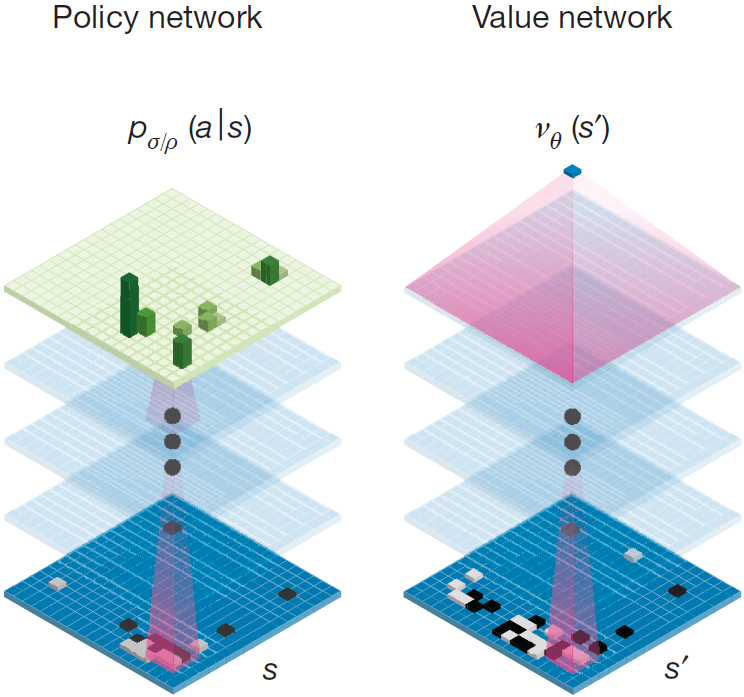
\includegraphics[height=.85\textheight]{../img/policy_and_value_network.png}
      \end{center}
    \end{frame}

    \begin{frame}{Rollout policy}
      \todo
    \end{frame}

    \begin{frame}{SL policy networks}
      \todo
    \end{frame}

    \begin{frame}{RL policy networks}
      \todo
    \end{frame}

    \begin{frame}{Value network}
      \todo
    \end{frame}

    \begin{frame}{MCTS with neural networks (1/4)}
      \begin{center}
        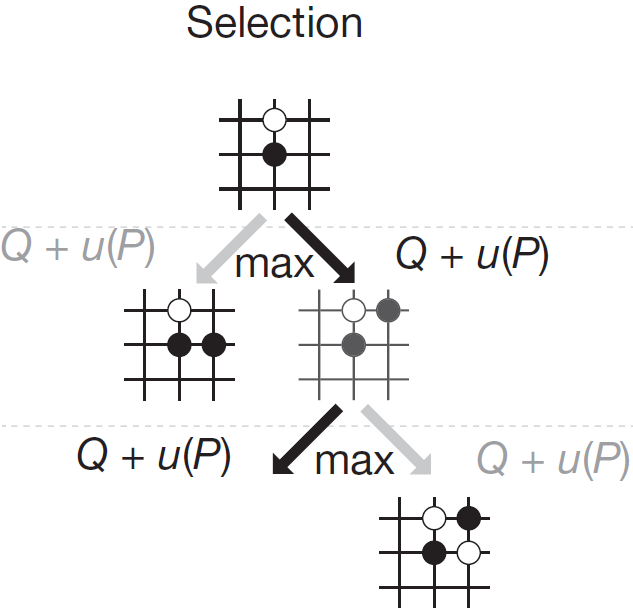
\includegraphics[height=.85\textheight]{../img/MCTS_selection.png}
      \end{center}
    \end{frame}

    \begin{frame}{MCTS with neural networks (2/4)}
      \begin{center}
        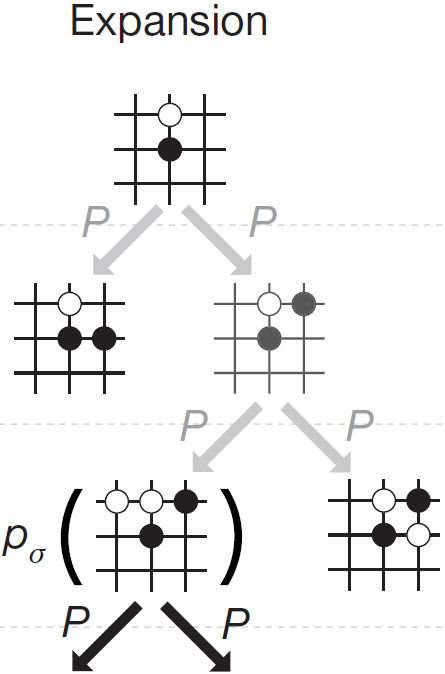
\includegraphics[height=.85\textheight]{../img/MCTS_expansion.png}
      \end{center}
    \end{frame}

    \begin{frame}{MCTS with neural networks (3/4)}
      \begin{center}
        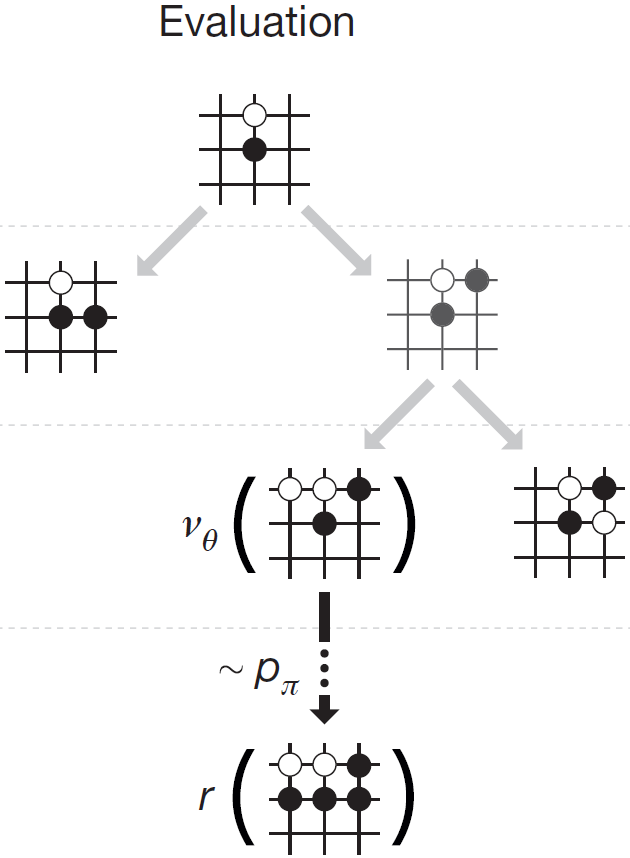
\includegraphics[height=.85\textheight]{../img/MCTS_evaluation.png}
      \end{center}
    \end{frame}

    \begin{frame}{MCTS with neural networks (4/4)}
      \begin{center}
        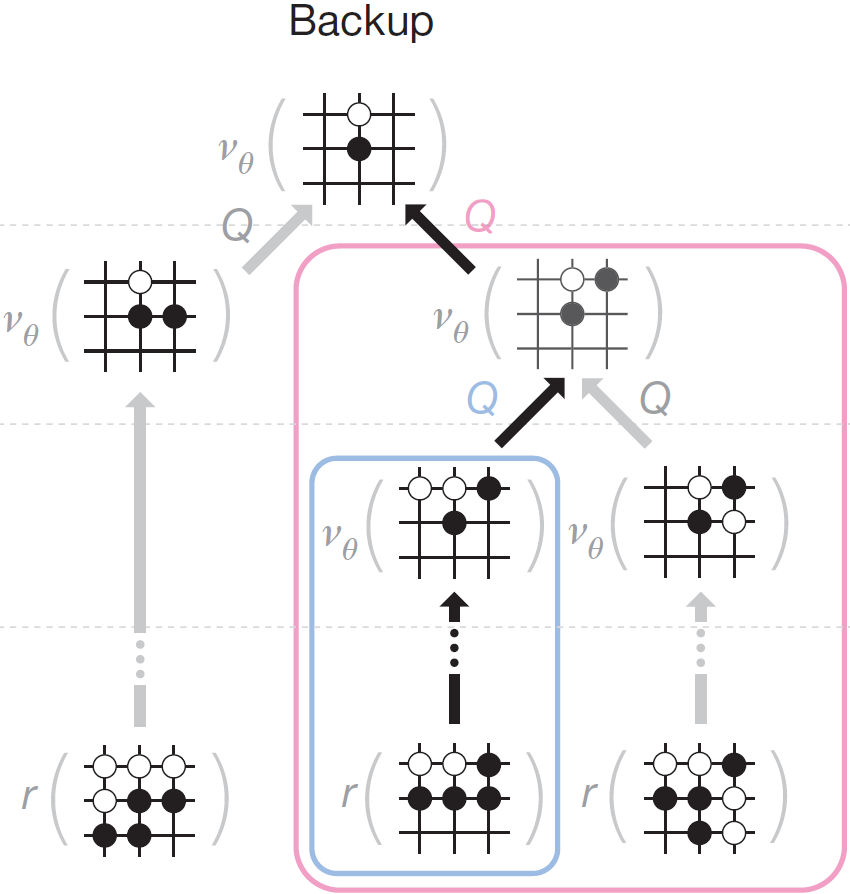
\includegraphics[height=.85\textheight]{../img/MCTS_backup.png}
      \end{center}
    \end{frame}

    \begin{frame}{Scalability}
      \todo
    \end{frame}
  }

%%%%%%%%%%%%%%%%%%%%%%%%%%%%%%%%%%%%%%%%%%%%%%%%%%%%%%%%%%%%%%%%%%%%%%%%%%%%%%%%

  \section{Results: the strength of AlphaGo}

  \begin{frame}{Tournament with other Go programs}
    \todo
  \end{frame}

  \begin{frame}{AlphaGo vs. Fan Hui}
    \todo
  \end{frame}

  \begin{frame}{AlphaGo vs. Lee Sedol}
    \todo
  \end{frame}

%%%%%%%%%%%%%%%%%%%%%%%%%%%%%%%%%%%%%%%%%%%%%%%%%%%%%%%%%%%%%%%%%%%%%%%%%%%%%%%%

  \section{Conclusion}

  \begin{frame}{Discussion}
    \todo
  \end{frame}

  \begin{frame}[standout]
    \begin{center}
      Thank you!
      \pause

      Questions?
    \end{center}
  \end{frame}

%%%%%%%%%%%%%%%%%%%%%%%%%%%%%%%%%%%%%%%%%%%%%%%%%%%%%%%%%%%%%%%%%%%%%%%%%%%%%%%%

  \appendix

  \begin{frame}[standout]
    Backup slides
  \end{frame}

  \begin{frame}{Further reading}
    AI:
    \begin{itemize}
      \item \textbf{Singularity} \url{http://waitbutwhy.com/2015/01/artificial-intelligence-revolution-1.html} + Part 2
    \end{itemize}

    \todo
  \end{frame}

  \begin{frame}[allowframebreaks]{References}
    \tiny
    \printbibliography[heading=none]
  \end{frame}

\end{document}
